\documentclass{article}
\usepackage{tikz}
\usetikzlibrary{calc,arrows}

% https://tex.stackexchange.com/questions/155401/connection-handshake-diagram-with-tikz

\begin{document}
\begin{center}
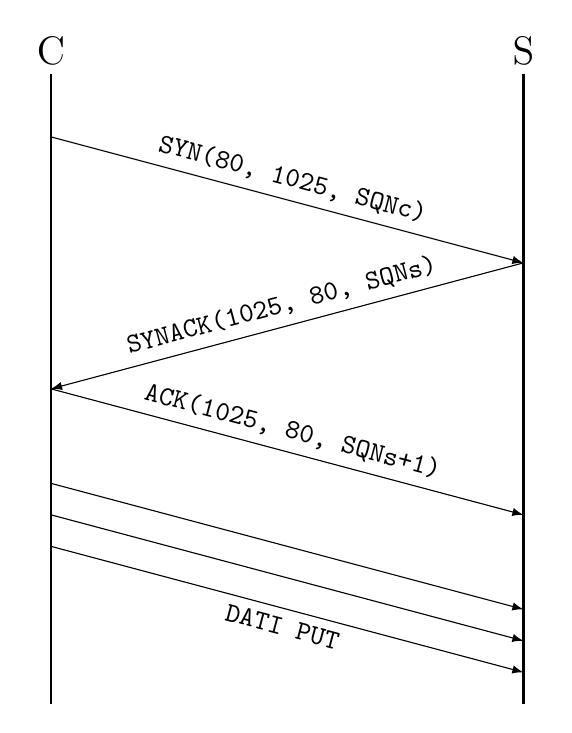
\begin{tikzpicture}[>=latex]

	% define the coordinates of client timeline
	\coordinate (A) at (0,8);
	\coordinate (B) at (0,0);
	
	% defien the coordinates of server timeline
	\coordinate (D) at (6,0);
	\coordinate (C) at (6,8);
	
	% draw client and server timeline
	\draw[thick] (A)--(B) (C)--(D);
	% label it on the top	
	\draw (A) node[above]{\Large C};
	\draw (C) node[above]{\Large S};

	\coordinate (E) at ($(A)!.1!(B)$);
	\draw (E) node[left]{
		\begin{tabular}{r}
			%\textit{}\\
			%\verb$$
		\end{tabular}
	};

	\coordinate (F) at ($(C)!.3!(D)$);
	\draw (F) node[right]{
		\begin{tabular}{l}
			%\verb$$\\
			%textit{}
		\end{tabular}
	};	
	\draw[->] (E) -- (F) node[midway,sloped,above]{\verb$SYN(80, 1025, SQNc)$};

	\coordinate (G) at ($(A)!.5!(B)$);
	\coordinate (G1) at ($(A)!.65!(B)$);
	\coordinate (G2) at ($(A)!.70!(B)$);
	\coordinate (G3) at ($(A)!.75!(B)$);
	\draw (G) node[left]{
		\begin{tabular}{l}
			%\verb$$
		\end{tabular}
	};
	\draw[->] (F) -- (G) node[midway,sloped,above]{\verb$SYNACK(1025, 80, SQNs)$};

	\coordinate (H) at ($(C)!.7!(D)$);
	\coordinate (H1) at ($(C)!.85!(D)$);
	\coordinate (H2) at ($(C)!.90!(D)$);
	\coordinate (H3) at ($(C)!.95!(D)$);
	\draw (H) node[right]{
		\begin{tabular}{l}
			%\verb$$
		\end{tabular}
	};
	\draw[->] (G) -- (H) node[midway,sloped,above]{\verb$ACK(1025, 80, SQNs+1)$};
	
	\draw[->] (G1) -- (H1) node[midway,sloped,above]{\verb$$};
	\draw[->] (G2) -- (H2) node[midway,sloped,above]{\verb$$};
	\draw[->] (G3) -- (H3) node[midway,sloped,below]{\verb$DATI PUT$};	
	
\end{tikzpicture}
\end{center}
\end{document} 